%%% -*-LaTeX-*-
%%% ====================================================================
%%% This is a sample top-level LaTeX-2e file for typesetting a thesis
%%% or dissertation at the University of Utah.  Most students find it
%%% convenient to start with a COPY of this file as a template, and
%%% then alter that copy to match their needs.
%%%
%%% There is an associated Unix Makefile that can be similarly
%%% customized, and then the only command ever needed to typeset the
%%% complete thesis is the single word "make".  Of course, during
%%% writing and typesetting, not all of the steps are needed, so
%%% often, one can just name a convenience target such as "make
%%% dvi-pass" or "make pdf-pass" to do just a single pass of LaTeX and
%%% BibTeX.
%%%
%%% There should be no, or very few, macro definitions in this file;
%%% any needed belong in a private style file, called mythesis.sty,
%%% and input below after all other packages.  The bulk of this file
%%% should just be command invocations, and any arguments that they
%%% need.
%%%
%%% We exploit the fact that TeX ignores spaces after command names to
%%% line up arguments for better readability.
%%%
%%% Each chapter should be a separate complete file, so that you can
%%% insert a command like \includeonly{chap_intro} before the first
%%% \include{chap_xxx} command to avoid typesetting all but the
%%% chapter that you are currently working on, to save time.
%%%
%%% Remember that occupants of job positions change jobs from time to
%%% time: YOU are responsible for ensuring correct names of all humans
%%% mentioned in this file!
%%%
%%% [16-Mar-2016]
%%% ====================================================================

\documentclass[11pt,Chicago]{uuthesis2e}
\paperheight 11in
\paperwidth 8.5in

%%% Undefine two macros from uuthesis2e.cls that conflict with
%%% definitions in amsthm.sty that fail to check for prior definitions!
%%% NB: The amsthm package refines the LaTeX theorem environment,
%%% and the uuthesis-color-headings wraps that definition, so the
%%% amsthm package must be read first!
\let \proof    = \relax
\let \endproof = \relax
\usepackage {amsthm}


%%% ====================================================================
%%% Choose an alternate font family for the document if the TeX default
%%% of Computer Modern is not wanted:

\usepackage{mathpazo}
\usepackage{enumitem,amssymb}
\newlist{todolist}{itemize}{2}
\setlist[todolist]{label=$\square$}
\usepackage{pifont}
\newcommand{\cmark}{\ding{51}}%
\newcommand{\xmark}{\ding{55}}%
\newcommand{\done}{\rlap{$\square$}{\raisebox{2pt}{\large\hspace{1pt}\cmark}}%
\hspace{-2.5pt}}
\newcommand{\wontfix}{\rlap{$\square$}{\large\hspace{1pt}\xmark}}

%%% ====================================================================
%%% Some miscellaneous Utah- and student-specific settings:
%%%
%%% Chapter is one level, section and subsection are the next two levels.

\fourlevels

%%% ====================================================================
%%% The remaining packages are required by this particular thesis,
%%% but other theses will almost certainly need different packages:
%%%
%%% WARNING: MANY \LaTeX{} packages change dimensions, glue, and/or
%%% formatting styles, and such changes are likely to conflict with
%%% University of Utah Thesis Office requirements.  Therefore, minimize
%%% the number of packages that you include!

\usepackage {amsmath}
\usepackage {amssymb}
\usepackage {bm}
\usepackage {bibnames}
\usepackage {citesort}
\usepackage {graphicx}
\usepackage {graphpap}
\usepackage {longtable}
\usepackage {multirow}
\usepackage {tikz}
\usetikzlibrary {decorations.markings}
\usepackage {varioref}
\usepackage{review}

%%% ====================================================================
%%% Support for a subject index:

%% \usepackage {uuthesis-index}

%%% ====================================================================
%%% The various uuthesis-*.sty packages must come AFTER all other
%%% system-provided packages, so that they can correctly override
%%% settings from those packages.

%%% Include latest updates for 2016 (WARNING: the name is subject to
%%% change: see http://www.math.utah.edu/pub/uuthesis/ for the most
%%% current version.)

\usepackage {uuthesis-2016-h}  % MANDATORY package

%%% This is an OPTIONAL package that sets chapter and sectional headings
%%% in color:
%%% Use one or the other of these:
% \usepackage {color}
%%: \usepackage {uuthesis-color-headings}
%%: \definecolor{utahheadingcolor} {rgb}  {0.7, 0.0, 0.0}
%%: \definecolor{utahtheoremcolor} {rgb}  {0.490,0.149,0.804} % purple4
%%: \definecolor{utahtheoremcolor} {rgb}  {0.545,0.137,0.137} % brown4

%%% Here is another, and more convenient, way to define colors, via
%%% aliases of named colors in the X11-derived rgb.sty file

%%: \usepackage{coloralias}
%%: \definecoloralias{utahheadingcolor}{steelblue4}
%%: \definecoloralias{utahtheoremcolor}{hotpink3}

%%% The default heading color is utahred (defined by University Printing
%%% Services as 0.8 red, 0.0 green, 0.0 blue), but you could redefine
%%% that to, for example, a dark blue color, like this AFTER including
%%% the package:
%%%
%%%     \definecolor{utahheading}{rgb}{0,0,0.8}
%%%
%%% NB: Be careful with use of colors in typesetting, and in figures,
%%% because about 6 percent of the human male population is red/green
%%% color blind: they see those colors as shades of brown.  Red and
%%% blue, or blue and green, are better choices for choosing
%%% distinguishable colors.  Also, avoid light colors, especially
%%% yellow, because they are hard to see against white paper and
%%% screen backgrounds, and when printed on black-and-white printers,
%%% where they are rendered in gray, they may be too faint to read.

%%% ====================================================================
%%% Support for a subject index:
%
%: \usepackage {uuthesis-index}

%%% ====================================================================
%%% This single user-specific file is where all personal customizations
%%% and macro definitions should be placed, and it should come LAST,
%%% after ALL OTHER packages, in case it needs to override some of their
%%% definitions.

\usepackage {mythesis}

%%% ====================================================================
%%% The student-specific front matter fields are defined here:

\author                 {Ethan Kerzner}
\title                  {CREATIVITY WORKSHOPS FOR VISUALIZATION DESIGN STUDIES}
\thesistype             {proposal}

\dedication             {...}

%%% Most students need just a short degree name, like this:
\degree                 {Doctor of Philosophy}
%%% However, multiline degrees are possible, and are done like this:
%%% \degree                 {Doctor of Philosophy \\
%%%                         in \\
%%%                         Mathematical Physics}

%%% College- and Department-level definitions:
\approvaldepartment     {School of Computing}
\department             {School of Computing}
\graduatedean           {Alice B. Toklas}
\departmentchair        {Petrus Marcus Aurelius Featherstone-Hough}

%%% The graduate student's committee members:
\committeechair         {Miriah Meyer}
\firstreader            {Erik Brunvand}
\secondreader           {Jason Dykes}
\thirdreader            {Charles Hansen}
\fourthreader           {Alexander Lex}
\chairtitle             {Professor}

%%% NB: It is rare, but possible, for there to be two chairs, For
%%% example, one student had
%%%
%%% \committeechair{\mbox{\small Andrej Cherkaev and Andrejs Treibergs}}
%%%
%%% The \mbox{} ensures that line breaks cannot happen, and the \small
%%% is necessary to make the names fit on the Dissertation Approval form

%%% Dates that must be adjusted for each academic term, and be permitted
%%% according to the University of Utah Thesis Office:
\submitdate             {July 2017}
\copyrightyear          {2017}

%%% Dates on which committee members approved the thesis
\chairdateapproved      {30 May 2017}
\firstdateapproved      {30 May 2017}
\seconddateapproved     {30 May 2017}
\thirddateapproved      {30 May 2017}
\fourthdateapproved     {30 May 2017}

%%% ====================================================================
%%% Typesetting begins here:

\begin{document}

%% Comment out items by inserting a percent % character
\frontmatterformat
\titlepage
%\copyrightpage
%\dissertationapproval
\setcounter {page}     {2}             % UofU Thesis Office demands abstract on p. iii: start one lower
%\preface    {sources/00_abstract} {Abstract}
%\dedicationpage
\tableofcontents
%\listoffigures
%\listoftables
%
%%% Optional front matter page(s), made from source "notation.tex". If
%%% you don't need it, then comment out the \optionalfront command
%%% line!  The first argument is the (unnumbered) section header for
%%% the text supplied by the file input by the second argument; that
%%% file must NOT contain \chapter, \section, \subsection, \ldots{}
%%% sectioning commands.
%\optionalfront {Notation and Symbols} {\input{notation}}

%%% Uncomment this is you want the contents of acknowledge.tex typeset here.
%%% Note that both "Acknowledgement" and "Acknowledgment" are accepted
%%% spellings of that word.

% \preface{acknowledge}{Acknowledgements}

%%% Demonstrations of thesis typesetting features for the sample thesis.
%%% Once you have seen the examples, you can comment out this line.
%%: \optionalfront {Typesetting Experiments} {\input{samples.tex}}

\maintext       % Start normal page numbering: parts and chapters follow.

\pagestyle{headings} % NEW for sample-thesis-6

%%% -*-LaTeX-*-

\chapter{Introduction}

This proposed dissertation is about a framework that describes why and how to use creativity workshops in visualization design studies. In its formative work, we conducted two design studies where we used creativity workshops~\cite{Kerzner2017} and creativity methods~\cite{Kerzner2015} to quickly establish rapport with project stakeholders, to characterize the problems faced by analysts, and to explore solutions to those problems. We based our creativity methods and workshop on descriptions in the existing visualization literature, but we had many unanswered questions about how to effectively use them. To investigate these questions, we analyzed our use of creativity workshops and the experiences of 6 visualization researchers who have used creativity workshops in 15 projects. Based on this analysis and an extensive literature review, the primary anticipated contribution of this proposed dissertation is an actionable visualization creativity workshop framework grounded in creativity theory. It will describe theoretical and practical considerations of creativity workshops, including why it is important that they emphasize creativity and how to customize them to a specific project. This framework will provide guidance for designers to use creativity workshops in their own projects, connect that guidance with existing creativity theory, and identify opportunities for future research on creativity workshops in visualization design.

\section{Overview}

As visualization designers, we aim to create useful visualizations for data analysts in design studies~\cite{Sedlmair2012}. But creating useful visualizations is hard for a variety of reasons. Often, analysts cannot tell us what they want to do with visualization tools because humans struggle to communicate tacit knowledge~\cite{Polanyi1974}. This is further complicated by imperfect communication due to the specialized knowledge of both designers and analysts---we may not know their domain's vocabulary and they may not know what is possible with visualization~\cite{Wijk2006}. We also have to navigate the context where analysts work, accounting for the bureaucracy and political environment of their organizations~\cite{Sedlmair2010}. And we have to do all this while remaining productive as analysts expect to see rewards, often in the form of useful visualizations, for committing their limited time and energy to working with us~\cite{Sedlmair2010}. 

Visualization process models describe the steps of conducting a design study and define three categories of common challenges faced by designers: intellectual, organization, and interpersonal~\cite{McKenna2014,Munzner2009,Tory2004a,Lloyd2011,Sedlmair2010,Sedlmair2012}. \textbf{Intellectual challenges} relate to finding real needs for analysts and whether fulfilling those needs is an interesting visualization problem~\cite{Sedlmair2012}, such as eliciting requirements based on analysts' tacit knowledge~\cite{Polanyi1974}. \textbf{Organizational challenges} include political, bureaucratic, and administrative constraints, such as the ability to share sensitive data~\cite{Sedlmair2010} or the buy-in from management~\cite{Kerzner2015}. \textbf{Interpersonal challenges} focus on relationships or communication between individuals~\cite{Sedlmair2012}, for example, the amount of engagement that analysts have in the project~\cite{Sedlmair2010}. Failure to address any of these challenges undermines the project as seemingly small errors cascade through the design process~\cite{Munzner2009}.

The typical methods for navigating these challenges require significant time commitment, especially at the start of design studies. Commonly, designers use a mix of contextual inquiry and interviews for finding interesting domain problems~\cite{Sedlmair2012}. But these methods require the focused attention of analysts, potentially over multiple days~\cite{Holtzblatt1993}. This strains the collaboration as it requires a large time commitment before we can deliver useful visualizations. Large organizations complicate things further as we must work with a diverse set of analysts, requiring even more time and energy from them as we piece together the organization's goals from disparate perspectives~\cite{Kerzner2015}. 

Recently, designers used creativity methods and workshops to understand analysts' needs while accounting for intellectual, organization, and interpersonal challenges~\cite{Goodwin2013}. {\bf Creativity methods} are participatory activities that explicitly stimulate creative thinking \cite{Osborn1953}. {\bf Creativity workshops} are the structured use of one or more creativity methods, typically with about 10 participants in sessions ranging in length from 2 hours to 2 days~\cite{Jones2005}. The characteristics of creativity methods and workshops include repeated cycles of divergent and convergent thinking, interpersonal leveling, and open communication~\cite{Osborn1953}. Applied to design studies, they help designers and analysts explore the relevant problem and solution spaces~\cite{Goodwin2013}, aid in navigating organizational hierarchies~\cite{Kerzner2015}, and establish relationships with all project stakeholders~\cite{Goodwin2016}.

In the formative work of this proposed dissertation, we applied creativity methods and workshops in two design studies. In our first design study, we used creativity methods with defense analysts to make use of limited meeting time and to gain trust and buy-in from analysts' management~\cite{Kerzner2015}. In our second design study, we used a creativity workshop to understand the diverse analysis needs of neuroscientists and to engage all members of an academic laboratory~\cite{Kerzner2017}. 

We based our use of creativity methods and workshops on examples from the visualization literature~\cite{Goodwin2013,Dykes2010,Walker2013,Lloyd2011}. Although this literature reported enough information for us to use the methods, we did not understand how they could be tailored to our specific needs or why they were successful. The research reported on \emph{what} was done in the workshops. It left us to fill in the practical considerations, \emph{how} to use them, and the underlying theory, \emph{why} they were useful. 

This proposed dissertation will contribute a framework to demystify both the process and theory of using creativity workshops in design studies. The framework will be based on our analysis of qualitative data from 15 creativity workshops in a variety domains. It will also be grounded in creativity theory from an extensive literature review. It will answer questions that designers may have about creativity workshops, including: Why should we care about creativity in visualization design? What does creativity mean in this context? What are creativity methods and workshops? How do we decide if a creativity workshop will help our project? How do we plan a creativity workshop? How do we run a creativity workshop? And, how do we use the workshop output during the visualization design process?

Some of these questions have been addressed by the domains of creative problem solving, software engineering, and psychology, yet, this work fails to account for the nuances of visualization design. We will account for these nuances, including the use of specialized process models~\cite{Tory2004a}, the critical role of data early in the design process~\cite{Munzner2009}, the sharing of knowledge between designers and analysts~\cite{Wijk2006}, the fuzzy nature of visualization software requirements~\cite{Sedlmair2012}, the evolution of data and tasks that occurs throughout the project~\cite{McCurdy2016_Action}, and the organizational, intellectual and interpersonal challenges~\cite{Sedlmair2012}.

\section{Contributions}

This proposed dissertation's primary anticipated contribution is a {\bf visualization creativity workshop framework} to provide practical and theoretical guidance on their use in design studies. It will be supported by three main pillars: 1) reviewing literature on creativity workshops spanning various domains, including, psychology~\cite{Csikszentmihalyi1997,Gardiner1993,Kaufman2006,Sawyer2006,Sawyer2003}, problem solving~\cite{Michalko2006,Gordon1961,Couger1993,DeBono1983,Osborn1953,Miller1989}, and software engineering~\cite{Sanders2008,Dove2015,Sherwin2011,Muller1993,Sanders2010,Mahaux2014,Mahaux2014,Mahaux2007,Jones2008,Jones2007,Maiden2007,Maiden2005,Maiden2004}; 2) analyzing qualitative data collected from the experiences of 6 creativity and visualization experts\footnote{If you are curious: Miriah Meyer, Jason Dykes, Sara Jones, Sarah Goodwin, David Rogers (maybe), and Graham Dove (maybe)} who have used creativity methods and workshops in 15 projects~\cite{Dykes2010,Goodwin2013,Goodwin2016,Koh2011,Walker2013,Rogers2016,Jones2008,Jones2007,Nobre2017,Horkoff2015,Lisle2017,Dove2015}; and 3) analyzing our own experience using creativity methods and workshops in design studies~\cite{Kerzner2015,Kerzner2017}.

This proposed dissertation's secondary contributions are design studies where we used creativity methods and workshops. First, in a design study for defense analysts, we used creativity methods to make use of limited meeting time with our collaborators. This project's contributions include task analysis, data abstraction, and a visualization tool for analyzing spatial and non-spatial ballistic simulation data~\cite{Kerzner2015,Gribble2014}. Second, in a design study for neuroscientists, we used a full-day creativity workshop to expose shared needs and establish rapport with analysts. This project's contributions include a set of software requirements for multivariate graph analysis and two techniques for visualizing graph connectivity~\cite{Kerzner2017,Lauritzen2016}.

The secondary contributions provide important grounding for the proposed creativity workshop framework. Conversely, the creativity workshop framework synthesizes our experience with that of our collaborators and an extensive creativity literature review to propose best practices for using creativity workshops in design studies.

\section{Structure of this Proposal}

The remainder of this proposal includes related work, followed by a discussion of our three projects organized by time. Chapter~\ref{ch:related} contains work related to visualization creativity workshops. Chapter~\ref{ch:vulnerability} reports the design study with defense analysts. Chapter~\ref{ch:connectome} summarizes the design study with neuroscientists. Chapter~\ref{ch:creativity} outlines the proposed remaining work, the visualization creativity workshop framework. Finally, chapter~\ref{ch:conclusion} proposes a timeline for the remaining work. 


%The typical methods to navigate the organizational and intellectual challenges require significant time commitment, especially when working in large organizations. For example, contextual inquiry~\cite{Holtzblatt1993} requires the undivided attention of analysts and designers. 

%is generally recognized  increases linearly with the number of analysts in the organization. This also puts a burden on designers, as we try to piece together a big picture of domain goals based on analysts' disparate perspectives~\cite{Kerzner2015}.

%We also must establish rapport and trust with analysts while navigating the bureaucracy of their organization. 

%Typical methods to navigate these challenges require significant time commitment. We commonly rely on interviews and contextual inquiry to understand analysts' needs, but contextual inquiry, for instance, must be spread over days or weeks~\cite{Holtzblatt1993,Sedlmair2012}.  

%More specifically, in our experience conducting three design studies~\cite{Kerzner2015,Kerzner2016,Kerzner2017}, we were challenged early on to understand analysts' needs from their tacit knowledge, to find shared needs from diverse analysts, to establish rapport with analysts, to navigate the bureaucracy around data analysis, and to do so while under pressure to remain productive as analysts expected to see useful visualizations early in our projects.





%To create useful visualizations, we must understand the analysts' domain problem, relevant data, and analysis tasks~\cite{Munzner2009}. Based on that understanding, we create prototype visualizations. These prototypes start a design cycle, as analysts give feedback on prototypes that we use to better understand their needs~\cite{Tory2004}.

%Process models describe this cycle and its many nuances for visualization~\cite{Sedlmair2012,Munzner2009,Meyer2012,Koh2011,McKenna2014,Tory2004}. These models, however, often fail to help us start the design cycle. 

%In design studies, we aim to create visualizations for data analysts to solve problems~\cite{Sedlmair2012}. To do this, designers must navigate three types of challenges. grouped them into roughly three categories~\cite{Sedlmair2012}. First, intellectual challenges involve understanding analysts' needs and evaluating whether those needs are interesting visualization problems~\cite{Tory2004}. This often involves translating expert's specialized needs into visualization requirements~\cite{Wijk2006}. Second, organization challenges relate to navigating political, bureaucratic, and administrative constraints~\cite{Sedlmair2010}. Organizational challenges include working with sensitive data~\cite{Sedlmair2010} or establishing trust with analysts' management~\cite{Kerzner2015}. And, third, interpersonal challenges focus on relationships or communication between individuals~\cite{Sedlmair2012}, such as, for example, the amount of engagement that analysts have in the project~\cite{Sedlmair2010}. If we fail to address any of these challenges early on, it can cripple the project as seemingly small errors propagate through the design study~\cite{Munzner2009,Sedlmair2012}.

%Visualization process models guide us through design studies~\cite{Tory2004,Munzner2009,McKenna2014,Meyer2013}. These models describe cycles where we understand a domain problem, propose visualization solutions to that problem, and evaluate visualizations to better understand the problem~\cite{Tory2004}. But these models often fail to help us navigate the interpersonal, intellectual, and organizational challenges at the start of the design cycle. In our experience conducting two design studies~\cite{Kerzner2015,Kerzner2017}, we were challenged early on to understand analysts’ needs from their tacit knowledge, to find shared needs from diverse analysts, to establish rapport with analysts, to navigate the bureaucracy around data analysis, and to do so while under pressure to remain productive as analysts expected to see useful visualizations early in our projects.

%We navigated these challenges with creativity methods and workshops.  Creativity methods promote, among other things, interpersonal leveling, open communication, and repeated cycles of divergent and convergent thinking~\cite{Osborn1953}. Creativity workshops are the structured use of one or more creativity methods, typically with about ten participants in sessions of two hours to two days~\cite{Jones2005}. In our first design study, we used creativity methods with defense analysts to gain trust and buy-in from analysts and their managers~\cite{Kerzner2015}. In our second design study, we used a structured creativity workshop to understand the diverse needs of neuroscientists~\cite{Kerzner2017}. 


%In both of these projects, we used methods and workshops described in visualization literature, but we had to search 


%but we had many open questions about why they creativity worked, and how to make them work better.  


%Although they were successful, we had many unanswered questions spanning both the theoretical, why fostering creativity helped the design process, and practical, how to most effectively use creativity methods. After these projects, we began a collaboration with fellow visualization designers to share best practices for the use of creativity in visualization design. Based on our collective success, we believe that the visualization community would benefit from practical and theoretical guidance on how to use creativity workshops to start the design process by understanding user needs and building rapport with analysts. 

%Typical methods to navigate these challenges require significant time commitment. We commonly rely on interviews and contextual inquiry to understand analysts' needs, but contextual inquiry, for instance, must be spread over days or weeks~\cite{Holtzblatt1993,Sedlmair2012}. This is exacerbated when working with analysts in large organizations as we must piece together various analyst's perspectives to understand the overall domain goals~\cite{Kerzner2015,Sedlmair2010}. We also must establish rapport and trust with analysts while navigating the bureaucracy of their organization. If we fail to address any of these challenges early on, it can cripple the project as seemingly small errors propagate through the design process~\cite{Munzner2009,Sedlmair2012}.

% Generalize challenges
%More generally, the challenges we face early in the design process fit into three categories: intellectual, organization, and interpersonal. Intellectual challenges relate to finding real needs for analysts and whether fulfilling those needs is an interesting visualization problem~\cite{Sedlmair2012}, such as eliciting requirements based on analysts' tacit knowledge~\cite{Holtzblatt1993} and identifying shared needs from diverse analysts within an organization~\cite{Sedlmair2010}.  Organizational challenges include . 

%Methods that foster \emph{group creativity}---the collective creativity that emerges from the interaction and communication between group members~\cite{Sawyer2003}---

% Address challenges
%Creativity methods are useful for starting the visualization design process and navigating the intellectual, organization, and interpersonal challenges as seen by their successful use in a variety of projects~\cite{Kerzner2015,Kerzner2017,Goodwin2013,Goodwin2016,McKenna2014}. In our experience, they establish trust between analysts and designers while explicating the analysis needs of a domain: ``\emph{the structured format helped us to keep on topic and to use the short time wisely}" said an analyst we worked with ``\emph{it also helped us rapidly focus on what were the most critical needs going forward}.''


% Motivate
%This proposed dissertation is motivated by our success using creativity methods at the start of design studies with defense analysts~\cite{Kerzner2015} and neuroscientists~\cite{Kerzner2017}. 

% what will the framework do?
%This proposed dissertation will provide guidance on the practical and theoretical aspects of visualization creativity methods and their execution in creativity workshops. We will answer questions that designers may have about this topic, including: Why should we care about creativity in visualization design? What does creativity mean in this context? What are creativity methods and workshops? How do we decide if a creativity workshop will help my project? How do we plan a creativity workshop? How do we run a creativity workshop? And, how do we use the workshop output during the visualization design process? 

%Some of these questions have been addressed by the domains of creative problem solving, software engineering, and psychology, yet, work from these domains fail to account for the nuances of visualization design. We will account for these nuances, including the use of specialized process models~\cite{McKenna2014,Tory2004}, the critical role of data early on in the design process~\cite{Munzner2009,Lloyd2011}, the sharing of knowledge between designers and analysts~\cite{McCurdy2016,Wijk2006}, the fuzzy nature of visualization software requirements~\cite{Sedlmair2012}, and the evolution of data and tasks that occurs throughout the project~\cite{Sedlmair2012,McCurdy2016}.

%%% -*-LaTeX-*-

\chapter{Background and Related Work}
\label{ch:related}
This proposed dissertation is about a framework that describes how to use creativity workshops in visualization design studies. This chapter focuses on work related to creativity in this context. It summarizes theoretical creativity research, including definitions, models, and research methods. Next, it describes the origin and evolution of creativity workshops from problem solving to software engineering and visualization.

\section{Creativity Research}

Creativity research spans many domains, including philosophy~\cite{Poincare1982,Boden2004,Hadamard1945}, psychology~\cite{Sawyer2006,Plucker1999,Kaufman2006}, the arts~\cite{Dewey1934,Csikszentmihalyi1997,Sawyer2003}, business~\cite{Osborn1953,DeBono1983,VonOech1986}, and computer science~\cite{Shneiderman2005,Hewett2005,Boden2004}. Across these domains, researchers agree that {\bf creativity} is generating ideas that are new and useful, where both new and useful can be defined relative to an individual, to a group of people, or to all of humanity~\cite{Mayer1999}. 

The creativity in visualization design studies involves all of the project stakeholders working together to create a new and useful understanding of a domain problem, to propose new and useful visualization solutions for that problem, and to perform new and useful evaluations of those solutions~\cite{Sedlmair2012}. 

Both individuals and groups can be creative~\cite{Sawyer2003}. {\bf Individual creativity} refers to a single creator~\cite{Sawyer2006}. Although individual creators often communicate with others, this communication may be used selectively~\cite{Sawyer2006}. In contrast, {\bf group creativity} emerges from direct interactions between group members~\cite{Sawyer2003}. It is synergistic as the group creates ideas beyond what its members could do on their own. Individual and group creativity are complementary as group creativity often relies on the creativity of its individual members.

We are interested in group creativity as visualization design involves the project stakeholders creating ideas beyond what they could do on their own~\cite{Goodwin2013}. In other words, creativity workshops are about harnessing group creativity for visualization design.

There is extensive research on individual and group creativity spanning many domains. Next, we summarize common creativity models and research approaches that may be relevant to visualization creativity workshops. For a more complete overview of creativity research please refer to summaries of this field, including works by Sawyer~\cite{Sawyer2006,Sawyer2003},  Sternberg~\cite{Sernberg1999}, and Shneiderman~\cite{Shneiderman2005}.

\subsection*{Creativity Models}

Creativity models provide a useful vocabulary, yet they oversimplify human thought \cite{Sawyer2006}. The {\bf four stage model} describes a linear process of creativity~\cite{Hadamard1945,Poincare1982,Wallas1926}, though in reality it is more likely a cyclical and iterative process~\cite{Sawyer2006}. First, creators \emph{prepare}, learning domain concepts. Second, they \emph{incubate} ideas, forming new mental associations. Third, they have an \emph{insight}, generating a new idea. Finally, they \emph{verify} the idea, expressing and elaborating it. 

By expressing an idea, creators start a feedback loop where their actions change the environment, and this, in turn, changes their idea. For example, an artist's idea for a painting evolves as they see the impact of their paint on a canvas~\cite{Glaveanu2013}. The {\bf action theory of creativity} emphasizes the importance of this feedback loop~\cite{Sawyer2006}. 

The four stage model and action theory emphasize that creativity involves both \emph{thinking} and \emph{doing}, often through many interconnected cycles of ideation and expression. These models straddle philosophy and cognitive psychology as they distill human thought and interaction into simplified processes~\cite{Sawyer2006}. They are supported by various creativity research methods, described next. 

\subsection*{Research Methods}

The research methods most relevant to this proposed dissertation study creativity in the context where it occurs --- the real world, outside of controlled laboratory settings~\cite{Mayer1999}. Although these {\bf contextual creativity} approaches are criticized because they lack experimental control, they are ecologically valid and supported by a broad base of qualitative and quantitative data~\cite{Mayer1999}.

There are three broad types of contextual creativity research. Biographical researchers study creative individuals, often with interviews and observations~\cite{Csikszentmihalyi1997}.  Organizational researchers study creativity in large groups, such as businesses~\cite{Drucker1988}. This includes quantitative surveys to identify shared traits of creative organizations~\cite{Isaksen2000} and analyzing how leaders can foster creativity in their organization~\cite{Amabile2008}. Creativity support researchers synthesize the results of biographical, organizational, and other research, to understand how software can foster creativity, and make recommendations for software designers~\cite{Shneiderman2005}.

There are many other approaches to studying creativity that are not necessarily relevant to this proposed dissertation. The quantitative study of creativity --- such as measuring a group's creative output in a laboratory --- often lacks ecological validity and must be synthesized with contextual approaches to generate useful insight~\cite{Sawyer2006}. Additionally, biological~\cite{Martindale1999} and individual personalty methods~\cite{Plucker1999} attempt to explain creativity as an inherit feature of individuals, but have generally been unsuccessful~\cite{Sawyer2006}. Historical~\cite{Albert1999} and cultural creativity research ~\cite{Lubart1999} explains the change of our socio-cultural perspective of creativity over time. They show that the notion of creativity is a relatively new concept, having evolved in the mid-twentieth century.

From all these approaches to studying creativity, there is a general consensus on how creativity occurs~\cite{Mayer1999}. More specifically, creativity results from hard work, open communication, and many series of small but interconnected insights~\cite{Sawyer2006}. The best practices for fostering creativity, however, have changed over time. This can be seen in the evolution of applied creativity research, spanning the domains of problem solving, software engineering, and visualization. 

\section{Creativity for Problem Solving}

The idea of harnessing creativity methods for problem solving started in the fields of business, advertising, and engineering~\cite{Osborn1953}. These methods are based largely on analyzing personal experience, a form of contextual creativity research.

Explicitly using creativity to solve problems was first proposed by Osborn~\cite{Osborn1953}, where he coined the term \emph{brainstorming} with a militaristic definition of \emph{``using the \emph{brain} to \emph{storm} a creative problem - and to do so in a commando fashion, with each stormer audaciously attacking the same objective."} Effective brainstorming is the freewheeling generation of as many ideas as possible, followed by evaluation to identify the most promising ones. The Creative Problem Solving Group formalized these principles into a repeatable process that is used by consulting firms today~\cite{Isaksen2000}.

Related to brainstorming is Synectics, which encourages problem solving through structured workshops consisting of three phases~\cite{Gordon1961}. First, workshop participants explore a given problem, often in terms of needs or wishes. Next, participant use the ideas as \emph{springboards} for in-depth discussion and elaboration. Third, participants evaluate the ideas and execute the more promising ones. The Synectics methodology has been adopted by various consulting and training companies~\cite{Nolan2003}.

Many consultants have also written books about their experience using creativity for problem solving, often in business settings. de Bono~\cite{DeBono1983} emphasizes ideation through suspending judgment and restructuring ideas. Similarly, von Oech~\cite{VonOech1986,VonOech1988} encourages creators to gain new perspectives on their problems with structured methods. Miller~\cite{Miller1989} proposes that creators should balance analytic methods, such as listing assumptions, with intuitive methods,such as brainstorming.

Many aspects of creativity for problem solving are still in use today, such as suspending judgment~\cite{Osborn1953}, encouraging the use of metaphors and analogies~\cite{Gordon1961}, and promoting reflection~\cite{DeBono1983}. However, on their own these methods are not immediately applicable to visualization design. They assume the workshop participants have sufficient knowledge to reach a valid solution whereas visualization designers recognize that they must establish shared knowledge of visualization and their collaborator's domain for a successful project~\cite{Wijk2006}. 

\section{Creativity Workshops in Software Engineering}

Software requirements engineers translate the specialized knowledge of project stakeholders into concrete requirements. This is a creative process as the engineers must create requirements that define useful software~\cite{Robertson2002}. In some projects, engineers use creativity workshops to elicit needs from project stakeholders~\cite{Jones2005}. These workshops range in duration from 0.5 to 2 days, involve 8 to 24 participants, and typically output hundreds of ideas about software requirements ~\cite{Jones2007}.

The creative problem solving literature provides a foundation for creativity workshops in this domain.  Maiden et al.~\cite{Maiden2004} reported the first creativity workshop in software engineering. It was a two day workshop to create requirements for aircraft scheduling software, using methods to encourage analogical thinking --- similar to Synectics~\cite{Gordon1961}. Another two day workshop run by Maiden et al.~\cite{Maiden2007} used repeated cycles of divergent and convergent thinking --- similar to Creative Problem Solving~\cite{Osborn1953} --- to understand requirements for airspace management software. Similarly, Jones et al.~\cite{Jones2007} used a creativity workshop to create requirements for e-learning software also following a diverge-converge pattern.

Creativity research in software engineering also examines the theory behind workshops. Mahaux et al.~\cite{Mahaux2013,Mahaux2014} describe and validate a set of factors that influence creativity in groups of software engineers, but this work falls short of prescribing best practices for fostering creativity. Recently, Maiden et al.~\cite{Maiden2010} mapped the use of creativity requirements workshops to those of creative problem solving to identify areas for future work. 

There has also been work to analyze the creativity methods for requirements engineering. Horkoff et al.~\cite{Horkoff2015} categorize methods by the structure of their output, arguing that more structured output is effective for engineers. Biskjaer et al.~\cite{Biskjaer2017} propose a framework for analyzing creativity methods based on certain attributes, including their structure and their use of divergent or convergent thinking. And Grube et al~\cite{Grube2008} categorize methods based on where they should be used in the design process. While these works provide important classification of creativity methods, they do not address the challenges of assembling creativity methods into a coherent workshop. 

Moreover, research in software engineering does not immediately apply to visualization design. In this domain, creativity workshops are often part of larger requirements engineering methodologies~\cite{Jones2005}. Their outputs are used to generate formal requirements for software developers~\cite{Maiden2005}. In contrast, visualization software requirements are often ill defined~\cite{Sedlmair2012} and evolve throughout the project~\cite{McCurdy2016_Action}.

\section{Creativity Workshops for Visualization}

Visualization is generally seen as a creative problem, where creativity is needed to explore a broad space of ideas before winnowing down to the more promising ones~\cite{Munzner2009,McKenna2014,Sedlmair2012}. The explicit use of creativity methods in visualization design evolved independently but in parallel to their use in software engineering. 

In visualization, creativity methods and workshops were first described as part of design studies. Dykes et al.~\cite{Dykes2010} used a full day workshop to understand the visualization needs of geographic information systems analysts. Walker et al.~\cite{Walker2013} used a similar workshop to quickly understand the needs of defense analysts. Kerzner et al.~\cite{Kerzner2015} used creativity methods to engage analysts and their managers in a large organization. These projects did not describe their work as creativity methods or workshops, but in retrospect these are early examples of explicitly fostering creativity for visualization design.

Goodwin et al.~\cite{Goodwin2013} introduced the term \emph{creativity workshop} to visualization. They customized software engineering creativity workshops for a design study with energy analysts. Kerzner et al.~\cite{Kerzner2017} applied the same workshop structure to understand the needs of neuroscientists. Recently, Goodwin et al.~\cite{Goodwin2016} again used a similar workshop structure to understand the needs of constraint programmers.

Different creativity workshop structures have also been used in visualization research. Nobre et al~\cite{Nobre2017} used a two hour workshop to understand how genealogists could use their visualization software. Lisle et al.~\cite{Lisle2017} used a two day creativity workshop to find opportunities for a collaboration between visualization designers and evolutionary biologists. Rogers et al.~\cite{Rogers2016} brought together visualization designers to explore potential solutions to specific problems in the domains of civil engineering and oceanography.

Despite these repeated success, understanding how to use creativity workshops requires that designers must piece together disparate information from the literature of visualization, software engineering, problem solving, and psychology. There are no guidelines nor best practices for applying creativity workshops to visualization design. This proposed dissertation will identify such best practices, based on the analysis of \emph{every} visualization project mentioned in this section. Before proposing the framework, we present our completed formative work that used creativity methods and workshops in two design studies.
\chapter{Completed Formative Work: Visual Vulnerability Analysis}
\label{ch:vulnerability}

The first design study of this proposed dissertation is a 15-month remote collaboration with defense analysts at the U.S. Army Research Laboratory. They were were trying to improve the safety of military vehicles using ballistic simulations to understand how vehicles may be vulnerable. Based on their findings, they would recommend changes to vehicle design. We worked with three analysts to understand how they used ballistic simulation results and we created a visualization tool to support their analysis. 

%They worked with ballistic simulation data: output attributes of physics-based simulations, 3D computer aided design models, and abstract relationships between vehicle components. Analysts used insights from this data to debug simulation inputs, identify components likely to be damaged, plan live-fire testing, and ultimately make recommendations about vehicle design. 

This design study is a formative project of this proposed dissertation as we used creativity methods to understand our collaborators' needs given limited time to meet in person. The creativity methods revealed visualization needs at a high level of abstraction that we investigated in more detail using contextual inquiry. This project also provides qualitative data to support the proposed creativity workshop framework. 

In this chapter we describe the project's contributions, summarize the resulting visualization tool, reflect on our use of creativity methods, and list the project's publications.

\section{Contributions}

This design study had three primary contributions: 1) a problem characterization, data abstraction, and task analysis for the domain of vulnerability analysis; 2) ShotViewer, a validated software prototype for visual vulnerability analysis; and 3) a reflection on creativity methods that will be part of this proposed dissertation's visualization creativity workshop framework.

It also had three secondary contributions: 1) a strategy for exploiting view-design parallelism while creating multiview visualizations based on a reflection of our work; 2) four recommendations for conducting design studies in large organizations with sensitive data; and 3) an algorithm that increased the computational efficiency of the ballistic simulations.

In the next section, we briefly describe the primary contributions. Please see the publications at the end of this chapter for more details about all of the contributions. 

\section{ShotViewer: Visualizing Ballistic Simulations}

We worked with analysts who were trying to understand the results of ballistic simulation software. The simulations are best explained by looking at its origins: an optical ray tracer~\cite{Butler2007}. Ray tracers compute photon paths through an environment, shade surfaces using physically-based lighting models, and output pixel color based on primary visibility rays. Ballistic simulations replace photons with {\bf shots}, a projectile being simulated, compute energy transfer using physically-based penetration models, and simulate the shot's impact on vehicle functionality using fault trees~\cite{SURVICEEngineering2013}. Historically, the simulations output statistical summaries such as the total vulnerable area of a vehicle, but these summaries have a nebulous definition that make it almost impossible to reason about why a vehicle may be vulnerable~\cite{Guber1967}. 

The goal of this work was to create tools that visualize the rich and descriptive simulation data to supplement the numerical summary values. Through creativity methods and contextual inquiry, we discovered that analysts needed to compare the simulations of a few shots simultaneously to explain trends and outliers in their data. Comparing shots was difficult, however, as it required the analysts to mentally combine three disparate datatypes: the physically-based penetration models, the 3D vehicle geometry, and fault trees --- abstract relationships between vehicle components representing its capabilities.

We developed ShotViewer to support analysis of this multityped data. ShotViewer, shown in Figure~\ref{fig:03_shotviewer}, displays shots with three linked, multiform views. The Shotline View (Figure~\ref{fig:03_shotviewer}a) displays the outputs of penetration models using a 2D parametrization of the shots. The Geometry View (Figure~\ref{fig:03_shotviewer}b) displays the 3D context of shots along with a subset of vehicle geometry. And the System View (Figure~\ref{fig:03_shotviewer}c) displays the impact of shots on the vehicle's components. Please see the publications at the end of this chapter for detailed descriptions of these views and a case study where ShotViewer was used to reason about vehicle vulnerability.

\section{Creativity Method Reflection}

We used creativity methods to navigate the challenges of working remotely with analysts who were part of a large and highly secure organization. There were organizational challenges as we had to excite analysts' managers because they were the organization's gatekeepers~\cite{Sedlmair2012}. There were interpersonal challenges as we tried to establish rapport with analysts given limited time to meet in person. And there were the standard intellectual challenges of finding an interesting visualization problem.

At the project's start we spent one week at our collaborator's offices where we used creativity methods in three half-day meetings with analysts and managers from various parts of the organization. The methods consisted of visualization awareness presentations~\cite{Lloyd2011} followed by brainstorming~\cite{Osborn1953}. We used visualization awareness to show our collaborators the potential applications of visualization. We used brainstorming to understand what our collaborators saw as their most pressing challenges. 

We engaged our collaborators with visualization awareness presentations. For example, when we presented a system for visualizing spatial and non-spatial biomechanical data developed by Keefe et al.~\cite{Keefe2009}, our collaborators saw the potential usefulness of a linked multiview system. A manager said that he wanted a similar system to explain ballistic simulation results as he said ``\emph{[the data behind simulations] is intelligible to only a few people and making sense of it is labor intensive."} 

Brainstorming helped us to discover the labor intensive parts of this analysis. All of the analysts had slightly different workflows and goals, but they used the same simulation software. During the brainstorming, all of the analysts had ideas about how visualization could help them reason about their combined spatial and non-spatial simulation input and output. This became the focus of our design study.

We investigated their analysis in detail using contextual inquiry~\cite{Holtzblatt1993}. The analysts and their managers were engaged with the contextual inquiry due, in part, to the creativity methods. After the contextual inquiry, we ultimately built ShotViewer to support the analysis of spatial and non-spatial ballistic simulation data.

\section{Conclusion and Publications}

In this design study, we used creativity methods to understand the needs of analysts in a large and highly secure organization. We then created and validated ShotViewer, a tool for visualizing multityped ballistic simulation data. 

This is a formative project of our proposed dissertation for two reasons. First, this project demonstrates that creativity methods and traditional contextual inquiry are complementary --- creativity methods provide an overview of domain challenges while contextual inquiry provides details about specific challenges. Second, it provides qualitative data to support the proposed creativity workshop framework. 

This project resulted in two publications. These papers will form this chapter in the proposed dissertation:

\begin{itemize}
    \item design study in Computer Graphics Forum, presented at EuroVis 2015 ~\cite{Kerzner2015}
    \item graphics algorithm in the Journal of Computer Graphics Techniques~\cite{Gribble2014}
\end{itemize}


\begin{figure}
 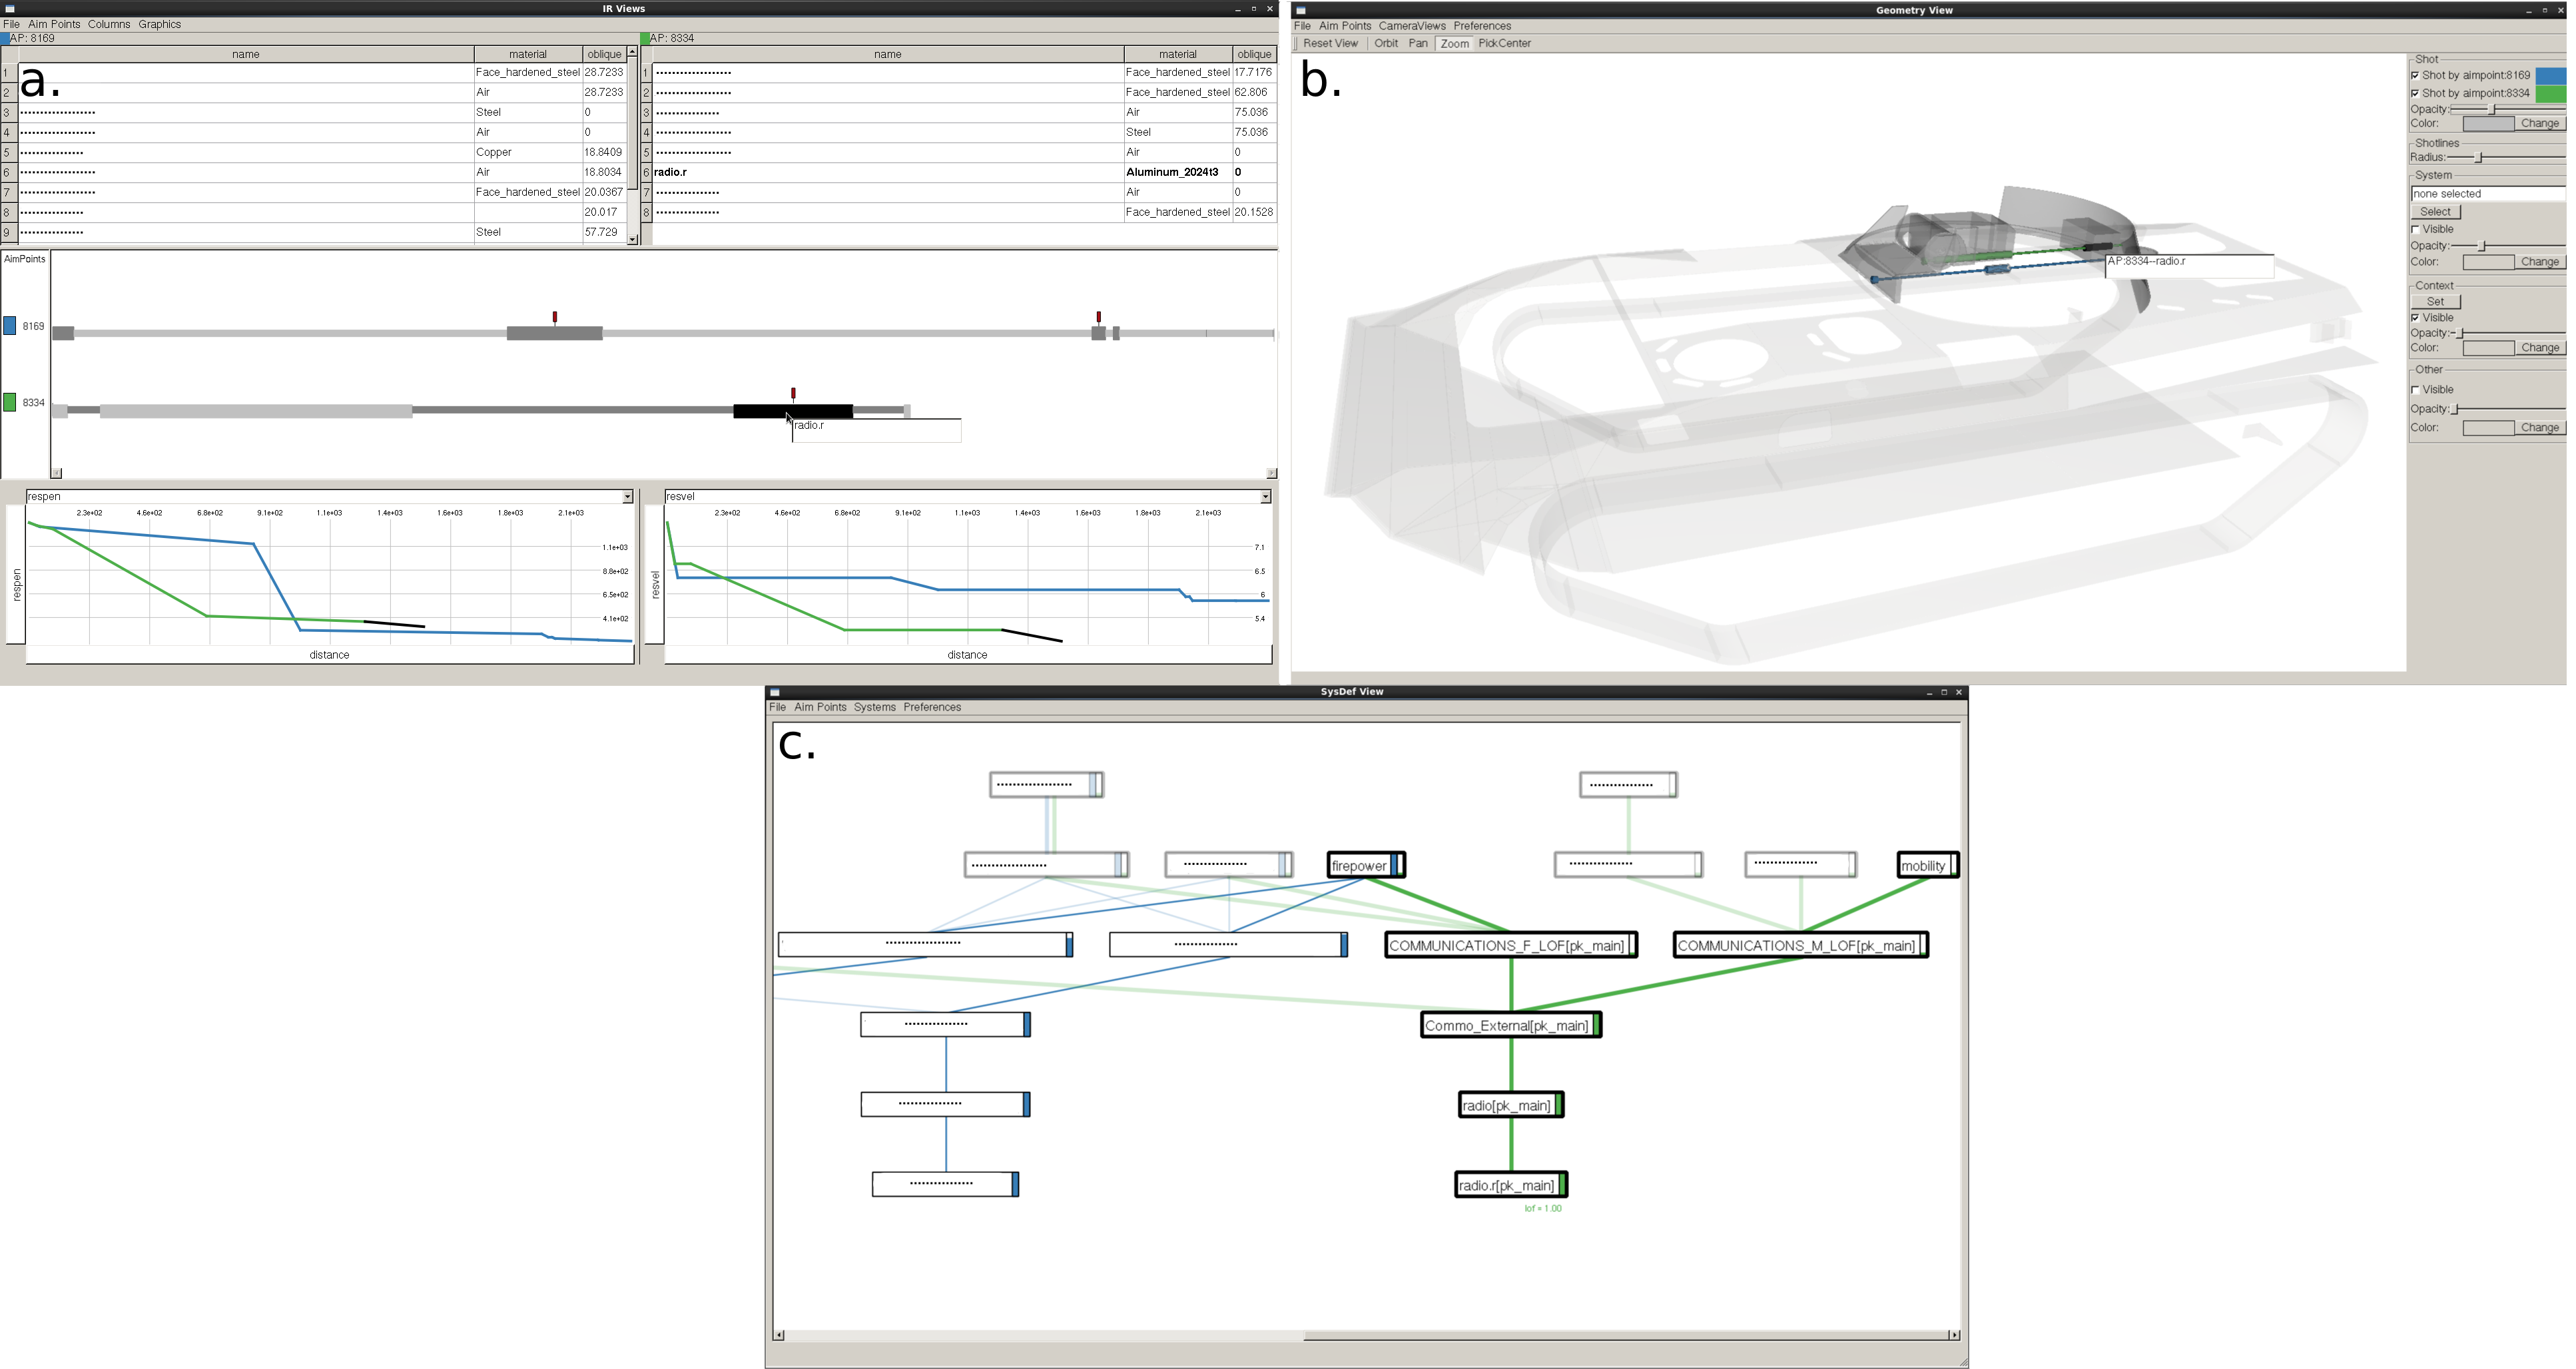
\includegraphics[width=\linewidth]{sources/figures/03_shotviewer}
  \caption{Shotviewer, software that supports visual analysis of spatial and nonspatial ballistic simulation data for vulnerability analysis. It consists of three linked views: a) the Shotline View displays an abstract representation of shots' paths through a vehicle; b) the Geometry View shows shots' 3D spatial context; and c) the System View visualizes the propagation of damage through a vehicle's systems. In this example, the green shot damages the vehicle's radio which impacts the vehicle's mobility and firepower capabilities.}
\label{fig:03_shotviewer}
\end{figure}
\chapter{Completed Formative Work: Connectome Visualization}
\label{ch:connectome}

The second design study of this proposed dissertation is a two year collaboration with neuroscientists who were trying to reverse engineer the retina at a cellular level. They were part of an academic laboratory at the Moran Eye Center, University of Utah. They worked on descriptive science but their long term goals were to understand neurodegenerative diseases and to create therapies for those diseases~\cite{Anderson2010}. We used a creativity workshop early in the project to learn how visualization could help their analysis. Based on this workshop's results, we focused on analyzing connectivity in large multivariate graphs --- our collaborators needed to analyze connectivity in a {\bf connectome}, a graph of neurons (nodes) connected by synapses (edges). To support their analysis, we created two new visualization techniques and realized those techniques in a prototype visualization tool.

This design study is a formative project of this proposed dissertation as it provides important practical experience using a creativity workshop. From this experience we started meeting with other visualization researchers to identify best practices for future creativity workshops. The anticipated creativity workshop framework resulted from those conversations. 

In the remainder of this chapter, we discuss this project's contributions, summarize the novel visualization techniques, reflect on the creativity workshop, and list the resulting publications.

\section{Contributions}

This project had five contributions: 1) a set of five requirements for visualization software to support connectivity analysis; 2) two new visualization techniques that summarize graph connectivity --- the connectivity matrix and the intermediate node table; 3) a prototype open source implementation of those techniques called Graffinity; 4) a reflection on the use of creativity workshops that inspired this proposed dissertation; and 5) the validation of our tools as they were used to discover new circuitry between cells in the retina~\cite{Lauritzen2016}.

In the next section, we briefly describe contributions \#2 and \#3. Please see the publications at this chapter's end for more details about all of the contributions.

\section{Graffinity: Visualizing Connectivity in Large Graphs}

We focused on supporting connectivity analysis, reasoning about the direct and indirect connections between nodes, based on paths, and potentially considering node and edge attributes~\cite{Lee2006}. For example, consider a large graph of airports (nodes) connected by flights (edges). An analyst may be interested in how the airports of two regions are connected, allowing for one or more layovers and accounting for attributes such as flight delay. Similarly, our collaborators wanted to understand how different sets of cells were connected by paths accounting for attributes such as cell type or synapse weight. 

Standard graph visualization techniques are not effective for connectivity analysis in large graphs. Node-link diagrams are helpful in judging connectivity but they degenerate to hairballs beyond about 50 nodes~\cite{Shneiderman2005}. Adjacency matrices also do not scale to large graphs and are only suitable to judge direct connections between nodes as they require tedious manual indirection between rows and columns to follow paths~\cite{Ghoniem2005}. 

A key approach to realize scalable graph visualization are queries: instead of displaying the whole graph, only a relevant subset is shown. Query-based techniques for analyzing connectivity in graphs, however, can also easily suffer from cluttering if the query result is big enough.

We proposed two new query-based visualization techniques that provide a scalable overview of graph connectivity without the need for manual tracing or indirection: the connectivity matrix and the intermediate node table. The connectivity matrix is an adjacency matrix generalized to show path connectivity. It summarizes paths based on their starting and ending nodes. The intermediate node table reveals information about the middle nodes that is hidden by the connectivity matrix. These two techniques provide a scalable overview of connectivity as seen in the prototype implementation of Graffinity, shown in Figure~\ref{fig:04_graffinity}. Please see our paper~\cite{Kerzner2017} for a full description of these techniques, example usage with a flight dataset, and validating case studies in connectomics analysis. 

\section{Creativity Workshop Reflection}

We started this collaboration with unstructured interviews and contextual inquiry~\cite{Holtzblatt1993} to understand our collaborator's analysis needs, but we found three limitations with these methods. First, we identified seemingly disparate needs as each analyst was interested in specific research questions. This is a common intellectual challenge when working in large organizations with specialized analysts~\cite{Sedlmair2010}. Second, we were not able to meet with senior analysts --- e.g., professors --- because they delegated our meetings to junior analysts --- e.g., post docs and graduate students. Third, we faced interpersonal challenges as some analysts were not necessarily engaged in our collaboration. We struggled to understand our collaborator's analysis needs due to these challenges.

We decided to use a creativity workshop to identify the shared needs of our collaborators. At first, we considered an unstructured meeting with analysts, but we did not know enough about the domain to plan one effectively. Instead, we ran a creativity workshop with eight of our collaborators, following the structure described by Goodwin et al.~\cite{Goodwin2013}. Its methods followed a diverge-converge pattern to explore a broad range of ideas and then to winnow the ideas and focus on the more interesting ones.

The workshop exposed shared analysis needs of our collaborators. In feedback on the workshop, the director of our collaborator's organization said \emph{``the structured meeting created consensus by exposing shared user needs."} We discovered that many analysts needed software to support reasoning about connectivity. The workshop also helped establish rapport and trust with our collaborators, as the director said the workshop's \emph{``interpersonal leveling and intense re-visiting of concepts made more team progress in a day than we make in a year of lab meetings."} Similarly, we estimated that the one day workshop produced data equivalent to six months worth of interviews and contextual inquiry.

\section{Conclusion and Publications}

In this design study, we proposed a set of requirements for connectivity analysis in large multivariate graphs. We created two new techniques to fulfill those requirements and implemented those techniques in a prototype tool called Graffinity. We validated Graffinity with case studies analyzing connectomics data.

This design study is a formative project of this proposed dissertation for two reasons. First, in our reflection on the workshop, we started working with six visualization researchers to find best practices for using creativity workshops in visualization design. Second, our use of a creativity workshop provides qualitative data for our proposed framework. 

This chapter will be formed from the following publications in the final dissertation:

\begin{itemize}
    \item technique paper in Computer Graphics Forum, presented at EuroVis 2017 ~\cite{Kerzner2017}
    \item results paper in the Journal of Comparative Neurology~\cite{Lauritzen2016}
\end{itemize}

\begin{figure}
 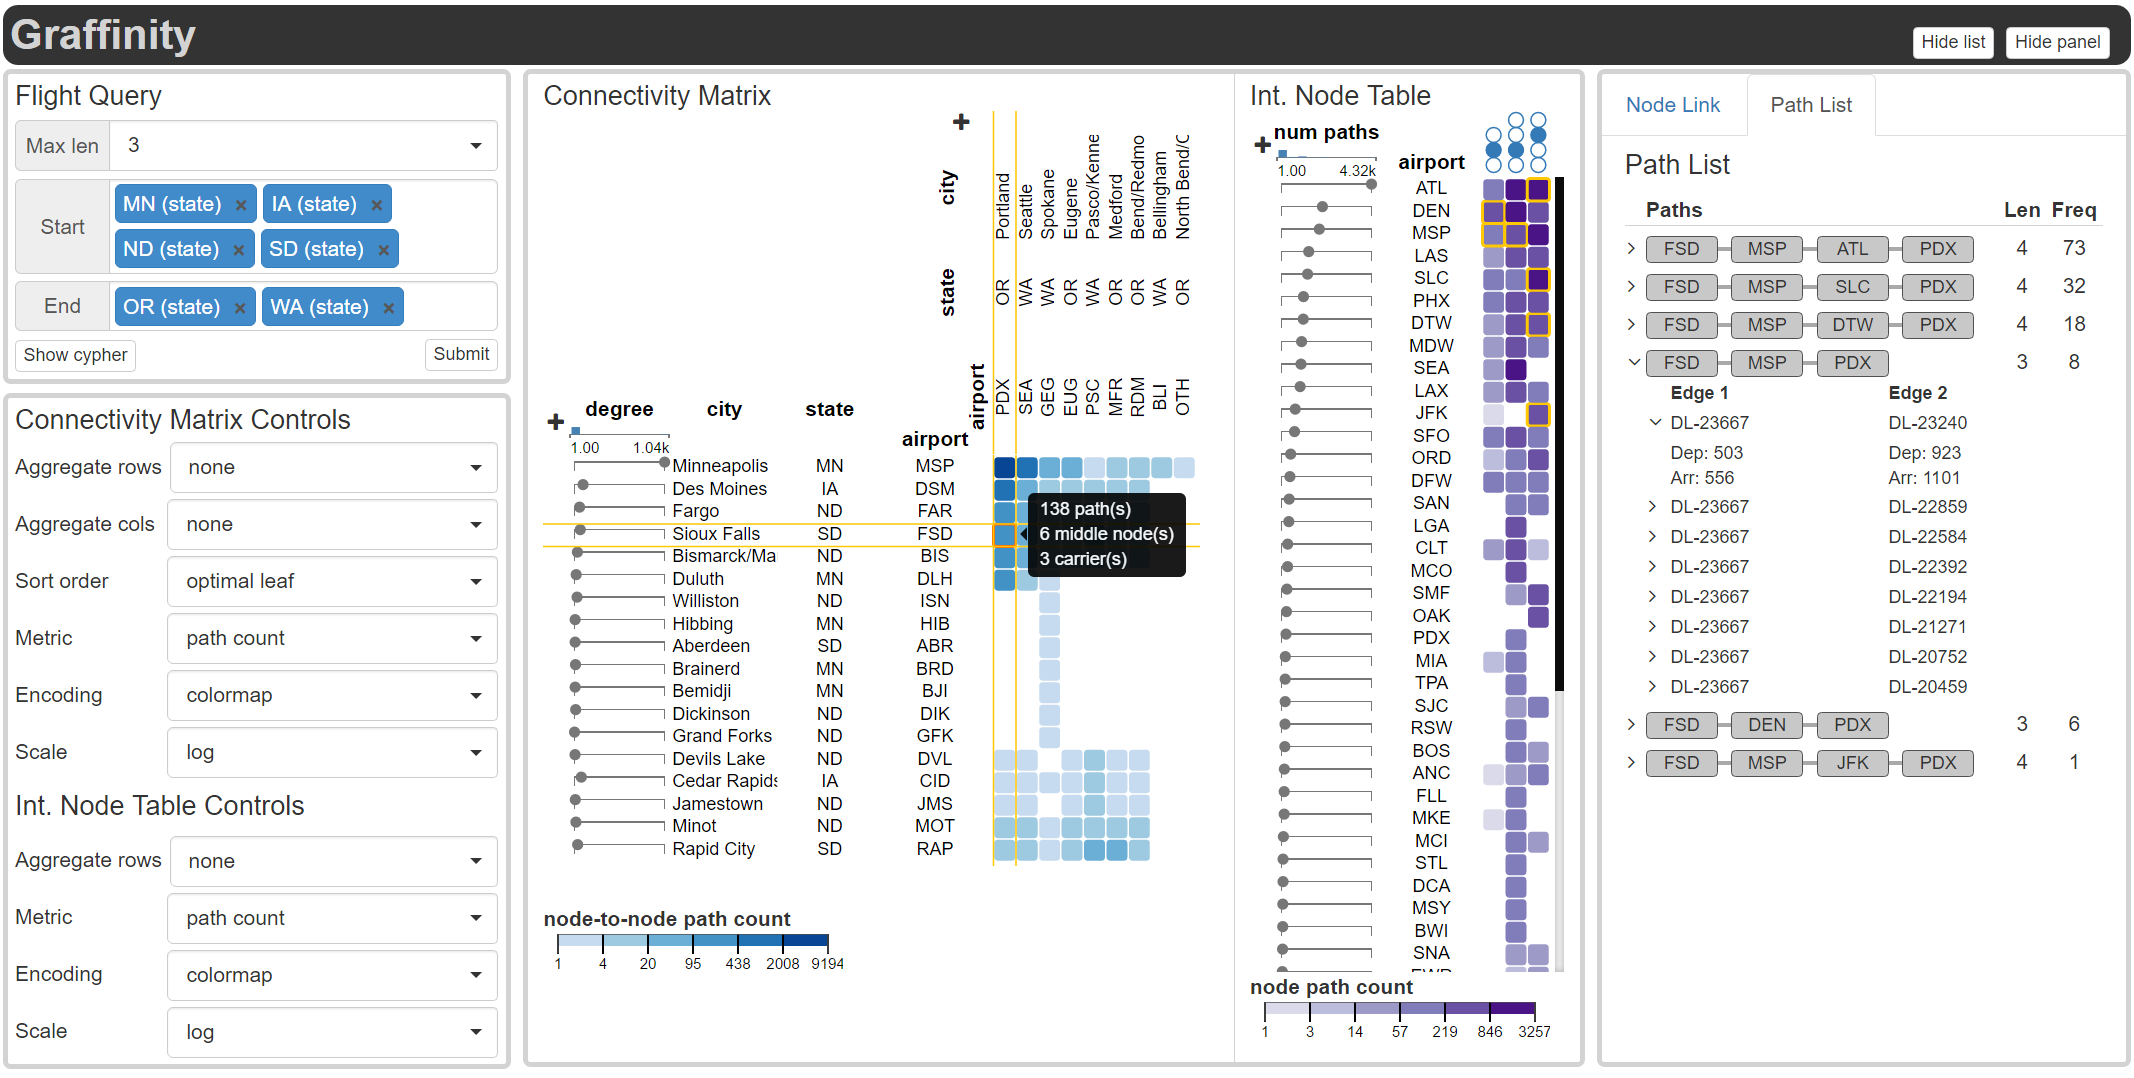
\includegraphics[width=\linewidth]{sources/figures/04_graffinity}
  \caption{Graffinity visualizing 11727 flight paths with length $\leq 3$ connecting states in the mid-western USA (Minnesota, Iowa, North Dakota and South Dakota) to states in the Pacific Northwest (Oregon and Washington). Graffinity consists of five views: the query interface, the connectivity matrix, the intermediate node table, and two views showing details about selected paths: the path list and the node-link view.  The 138 paths connecting the airport FSD (Sioux Falls, SD) to PDX (Portland, OR) are selected and displayed in the path list view.}
\label{fig:04_graffinity}
\end{figure}



%%% -*-LaTeX-*-

\chapter{Proposed Work: Visualization Creativity Workshops}
\label{ch:creativity}

The previous two chapters described design studies where we used creativity methods and workshops ad hoc. We ran them based on descriptions in the literature --- in retrospect, we did not understand why creativity is important, how to tailor creativity methods to fulfill our goals, nor the best practices for encouraging creativity. This is because there are currently no established guidelines or frameworks that describe how to use visualization creativity workshops. To explain the theory behind creativity workshops and to provide practical recommendations based on our experiences, we propose creating an actionable \emph{visualization creativity workshop framework} grounded in theory. 

In this chapter, we describe the research methods and data that we will use to create the framework. We outline the framework with set of 36 open questions. And we describe the project's remaining work. The anticipated outcome is a publication in IEEE Transactions on Visualization and Computer Graphics (IEEE TVCG).

\section{Data and Methods}

The proposed framework will be based in the analysis of creativity methods and workshops in a variety of projects. We are working with six creativity and visualization researchers who have also used creativity methods and workshops. Collectively with our collaborators, we have run more than 15 creativity workshops in a variety of domains and settings~\cite{Dykes2010,Goodwin2013,Goodwin2016,Koh2011,Walker2013,Rogers2016,Jones2008,Jones2007,Nobre2017,Horkoff2015,Lisle2017,Dove2015,Kerzner2017,Kerzner2015,Maiden2004,Maiden2005}. We gathered data from a subset of these workshops including the materials, agendas, artifacts, output, and impact on the project's final result. Analyzing these data will provide a practical foundation for our proposed framework.

The framework will also be grounded in creativity theory. We have reviewed literature related to creativity workshops in the fields of psychology~\cite{Csikszentmihalyi1997,Gardiner1993,Kaufman2006,Sawyer2006,Sawyer2003}, problem solving~\cite{Michalko2006,Gordon1961,Couger1993,DeBono1983,Osborn1953,Miller1989}, and software engineering~\cite{Sanders2008,Dove2015,Sherwin2011,Muller1993,Sanders2010,Mahaux2014,Mahaux2014,Mahaux2007,Jones2008,Jones2007,Maiden2007,Maiden2005,Maiden2004}.

We will create the framework through the qualitative analysis of data gathered from our experiences and our literature review. We will apply thematic analysis to identify overarching themes in our data~\cite{Braun2006}. But we also have tacit knowledge about creativity workshops that is not in the data. To capture this knowledge, we will use reflection, analyzing our experiences and proposing new insights based on that analysis~\cite{Boud1985}. More specifically, we will use collaborative reflection, analyzing many individuals' collective experience and articulating the insights of this analysis for future reference~\cite{Prilla2012}. We may also use qualitative analysis methods including open coding and grounded theory~\cite{Corbin1990}.

Through this analysis, we will create a framework that describes how and why to use creativity workshops in visualization design. As we have already started this analysis, we outline the framework in the next section.

%It is based on our experience and on existing theory. Over the past one and a half years, we carefully analyzed our experience with three workshops in more than one hundred hours of conversation~\cite{Goodwin2013,Goodwin2016,Kerzner2017}. And we reviewed literature related to creativity workshops in the fields of psychology~\cite{Csikszentmihalyi1997,Gardiner1993,Kaufman2006,Sawyer2006,Sawyer2003}, problem solving~\cite{Michalko2006,Gordon1961,Couger1993,DeBono1983,Osborn1953,Miller1989}, and software engineering~\cite{Sanders2008,Dove2015,Sherwin2011,Muller1993,Sanders2010,Mahaux2014,Mahaux2014,Mahaux2007,Jones2008,Jones2007,Maiden2007,Maiden2005,Maiden2004}. Through a form of thematic analysis~\cite{Braun2006}, including countless iterations on themes based on conversations with our collaborators, we synthesized the result of those conversations and literature review into a framework outline. 

%This outline will guide the creation of our complete framework as we work with collaborators to analyze our collective experience, including more than 12 creativity workshops a variety of domains~\cite{Dykes2010,Goodwin2013,Goodwin2016,Koh2011,Walker2013,Rogers2016,Jones2008,Jones2007,Nobre2017,Horkoff2015,Lisle2017,Dove2015}. We will use \emph{reflection}, analyzing our experience and proposing new insights based on that analysis~\cite{Boud1985}. More specifically, we will use \emph{collaborative reflection}, analyzing many individuals' collective experience~\cite{Prilla2012}. Collaborative reflection is different than informal discussions, for example, because it has explicit goals that include creating insights and articulating those insights for future reference~\cite{Prilla2012}. We may also use various qualitative research methods as part of our collaborative reflection, including grounded theory~\cite{Corbin1990} and thematic analysis~\cite{Braun2006}. 

%Collaborative reflection and literature review are accepted research methods for creating theoretical frameworks. Popular visualization process and decision models are based largely on these methods~\cite{Sedlmair2010,Munzner2009,Meyer2013,McKenna2014,Tory2004}. Also, collaborative reflection is a type of contextual creativity research as we analyze our data collected from experiences running creativity workshops in real projects~\cite{Sawyer2006}. Although contextual methods lack precise measurement and experimental control, they preserve ecological validity of observations~\cite{Mayer1999}. This is crucial for applied visualization research, as we aim to create insights that are transferable to future visualization projects~\cite{Sedlmair2012}. In our final framework, however, we will hedge the contributions according to the research methods used. Moreover, we hope that this framework provides appropriate language to enable future research on visualization creativity workshops.

\section{Visualization Creativity Workshop Framework}

The visualization creativity workshop framework consists of six stages that are based roughly on the steps that a designer would use in planning, running, and evaluating a workshop. The stages are: 1) {\bf motivate} the use of creativity workshops; 2) {\bf scope} the workshop focus and goals; 3) {\bf plan} the workshop methods and logistics; 4) {\bf run} the workshop; 5) {\bf analyze} the workshop output; and 6) {\bf reflect} on the workshop efficacy. For each of these stages, we describe its purpose, input, output, and a list of open questions that will need to be answered in our final framework.

These stages are an abstraction of a complex and messy process. They provide temporal constructs to organization the discussion of our experiences with creativity workshops. The remainder of this section outlines the six stages, followed by some general discussion questions that will need to be addressed in our publication.

\subsection*{Motivate}

The motivate phase is precondition to using creativity workshops. It is meant to convince designers that workshops are useful for design studies. The questions that a designer may have about this include:

\begin{enumerate}
    \item \emph{Why should I use a workshop? (Aren't interviews good enough?)}
    \item \emph{Why should my workshop be structured? (Can I just meet informally with my collaborators?)}
    \item \emph{What exactly does creativity mean in this context?}
    \item \emph{Why is it important that the workshops emphasize creativity?}
    \item \emph{Why do I need a \emph{visualization} creativity workshop framework? (Isn't the existing literature good enough? What are the nuances of visualization design that I need to account for in my workshop?)}
\end{enumerate}

\subsection*{Scope}

In the scope phase, we evaluate whether a workshop would be useful for a design study. Input to this phase is a design study with domain experts. Outputs from it include a workshop focus (what role it will serve in the design process e.g., to understand or to ideate~\cite{McKenna2014}) and goals (the stated reason for running the workshop). A designer may ask:

\begin{enumerate}
    \item \emph{Where is a good point in the design process to run a workshop? (Focus)}
    \item \emph{How much contextual knowledge do I need to run a workshop?}
    \item \emph{What can my collaborators and I expect to get from a workshop? (Goals)}
    \item \emph{Are my project constraints amenable to a workshop?}
\end{enumerate}

\subsection*{Plan}

In the plan phase, we assemble a workshop that fulfills the goals and focus while recruiting contributors. Input to this phase is a workshop scope --- the focus and goals. Output from it are a list of contributors (including facilitators, scribes, and participants), logistics (such as venue and duration), and methods (the activities planned for the workshop). The open questions are:

\begin{enumerate}
    \item \emph{Who should I recruit as contributors?}
    \item \emph{What should I consider in my logistics  --- venue and duration?}
    \item \emph{What are the different kinds of methods available for workshops?} %\ek{This question and the next one will probably be their own section in the final paper. There's a lot of interesting stuff we can talk about here: analytic vs intuitive, structured vs unstructured, paradigm preserving vs paradigm breaking, etc}
    \item \emph{How should I select methods to use in the workshop?}
    \item \emph{How should I consider the four stage model of creativity while planning my workshop?}
    \item \emph{How should I consider the action theory of creativity while planning my workshop?}
    \item \emph{Should I run a pilot workshop?}
\end{enumerate}

\subsection*{Run}

In the run phase, we execute the workshop and collect artifacts from it. Input to this phase is a workshop plan, including the contributors, logistics and methods. Output is a successfully executed workshop along with tangible and intangible results. A designer may ask:

\begin{enumerate}
    \item \emph{How should I prepare workshop contributors? (e.g., surveys of participants) }
    \item \emph{What are best practices for running the workshop?}
    \item \emph{How should I record ideas during the workshop?}
    \item \emph{How should I collect artifacts from the workshop?}
\end{enumerate}

\subsection*{Analyze}

In the analyze phase, we make sense of the tangible and intangible workshop results. Input to this phase are the results of a workshop that has recently been run. Output is actionable knowledge that fulfills the workshop focus and goals. The open questions are:

\begin{enumerate}
    \item \emph{What does the typical workshop output look like?}
    \item \emph{What are the different ways that I can make sense of workshop output?}
    \item \emph{How involved should workshop contributors be in analyzing the output?}
    \item \emph{How can I use workshop output in generative design methods?}
    \item \emph{How can I use workshop output in evaluative design methods?}
\end{enumerate}

\subsection*{Reflect}

In the reflect phase, we evaluate the efficacy of the workshop. Input to this phase are the scope, plan, execution and analysis. Output are insights for the visualization community, potentially transferable to future design studies. The open questions are:

\begin{enumerate}
    \item \emph{How should I collect feedback from workshop contributors?}
    \item \emph{How should I evaluate the workshop with respect to the scope and plan?}
    \item \emph{When and how should I evaluate workshop effectiveness?}    
    \item \emph{What is the role of quantitative/qualitative evaluation methods in our reflection?}
    \item \emph{What should I share about my workshop and reflection with the visualization community?}
\end{enumerate}

\subsection*{Discussion}

There are also interesting questions about creativity workshops that do not fit into the process of using them. These questions will be addressed in the discussion of our proposed work:

\begin{enumerate}
    \item \emph{What are the limitations of using creativity workshops?}
    \item \emph{How effective are creativity workshops with casual or non-expert users?}
    \item \emph{What is the relationship between visualization creativity workshops, participatory design, and co-design?}
    \item \emph{What is the relationship between visualization creativity workshops and agile development?}
    \item \emph{How do visualization creativity workshops apply to other areas of visualization research, such as technique or algorithm-driven work?}
    \item \emph{How can we validate the creativity workshop framework?}
\end{enumerate}

\section{Anticipated Publications and Remaining Work}

The remaining work of this project will expand this outline into a full framework for publication in IEEE TVCG. Writing this framework is an important part of our analysis as we will be forced to articulate our assumptions and ideas~\cite{Richardson2005}. We will also use the writing as a medium for collaborative reflection as we ask our collaborators to either support or refute what we have written. Through this writing, we will explicate our framework and identify best practices (or pitfalls) for applying creativity workshops to visualization design studies. The next chapter describes a more detailed timeline of the remaining work for this publication.
\chapter{Timeline}
\label{ch:conclusion}

This chapter provides a timeline of the work for this proposed dissertation. It starts with an overview timeline, summarizing the completed formative work and remaining work on the creativity workshop framework. It concludes with a detailed timeline of the proposed remaining project.

\section{Overview}

This proposed dissertation consists of three projects, two formative design studies followed by the creation of a theoretical framework. We ran the design studies over four years and have been working on the creativity workshop framework for the last two years in parallel with a design study. Here, we briefly describe each project, summarize the role of creativity methods and workshops in it, and list the resulting publications (first author publications are in bold).

\begin{todolist}
    \item[\done] \underline{\emph{{\bf Visual vulnerability analysis}, Sep-2013 -- Dec-'14 (1.5 years)}} --- a design study with defense analysts who were trying to understand the results of ballistic simulations.
    \begin{itemize}
        \item Creativity methods identified shared analysis needs and overcame challenges of working remotely with analysts in a highly secure and large organization
        \item Publications: {\bf design study in Computer Graphics Forum, EuroVis 2015~\cite{Kerzner2015}}; and algorithm in the Journal of Computer Graphics Techniques~\cite{Gribble2014}
    \end{itemize}
    
    \item[\done] \underline{\emph{{\bf Connectome visualization}, May-'15 -- Dec-'16 (1.5 years)}} --- a design study with neuroscientists who were analyzing the circuitry of cells in the retina.
    \begin{itemize}
        \item A creativity workshop established trust, fostered engagement, and exposed shared needs among diverse neuroscientists
        \item Publications: {\bf application/technique in Computer Graphics Forum, EuroVis 2017~\cite{Kerzner2017}}; and biology results in the Journal of Comparative Neurology~\cite{Lauritzen2016}
    \end{itemize}

    \item \underline{\emph{{\bf Visualization creativity workshop framework}, Jun-'15 -- present (2+ years)}} --- an actionable framework that provides theoretical and practical guidance on how to use creativity workshops in design studies.
    \begin{itemize}
        
        \item Analysis of creativity workshops in visualization design, based partly on creativity methods and workshops in the two aforementioned design studies.

        \item Anticipated publication: {\bf theory paper submitted to IEEE Transactions of Visualization and Computer Graphics (IEEE TVCG)}
    \end{itemize}
    
\end{todolist}

A majority of the remaining work involves writing the creativity workshop paper, which we describe in detail next. 

\section{Remaining Work}

We outlined the creativity workshop framework in chapter~\ref{ch:creativity} based on over two years of informal discussions and qualitative data analysis. Here is a detailed timeline of the completed work and proposed remaining work for this project.

\begin{todolist}
 
    \item[\done] \underline{\emph{Jun-'15 -- Jan-'17  (1.5 years)}} --- Discussed creativity workshops with collaborators informally. Attempted to write two papers on the topic, but ultimately decided that the papers were not yet ready for submission.
    
    \item[\done] \underline{\emph{Jan-'17 -- May-'17  (4 months)}} --- Created the current seven stage framework based on in-depth analysis of three workshops and an extensive literature review. 
    
    \item[\done] \underline{\emph{6-Jun-'17 -- 8-Jun-'17  (2 days, on-site in London)}} --- Met with collaborators, agreed on the seven stage framework as a foundation for our paper and outlined answers to questions in chapter~\ref{ch:creativity}.
    
    \item \underline{\emph{8-Jun-'17 -- 15-Aug-'17 (2 months)}} --- Draft answers to the questions outlined in chapter~\ref{ch:creativity} based on qualitative analysis of workshop data and collaborative reflection. Write a draft of the paper based on these answers.
    
    \item \underline{\emph{15-Aug-'17 -- 1-Sep-'17  (2 weeks)}} --- Seek external feedback on the paper and framework from other researchers\footnote{Francesca Samsel (Los Alamos National Lab), members of the Vis Design Lab, members of the giCentre}. Revise the framework based on this feedback.
    
    \item \underline{\emph{1-Sep-'17 -- 30-Sep-'17  (1 month)}} --- Write the final paper and submit to IEEE TVCG.

\end{todolist}

Following the paper submission, we will expand this proposal into a dissertation. Allowing for time to write and edit this dissertation, we hope to defend it by the end of the fall semester, 2017. 

%\begin{figure}
%\centering
% 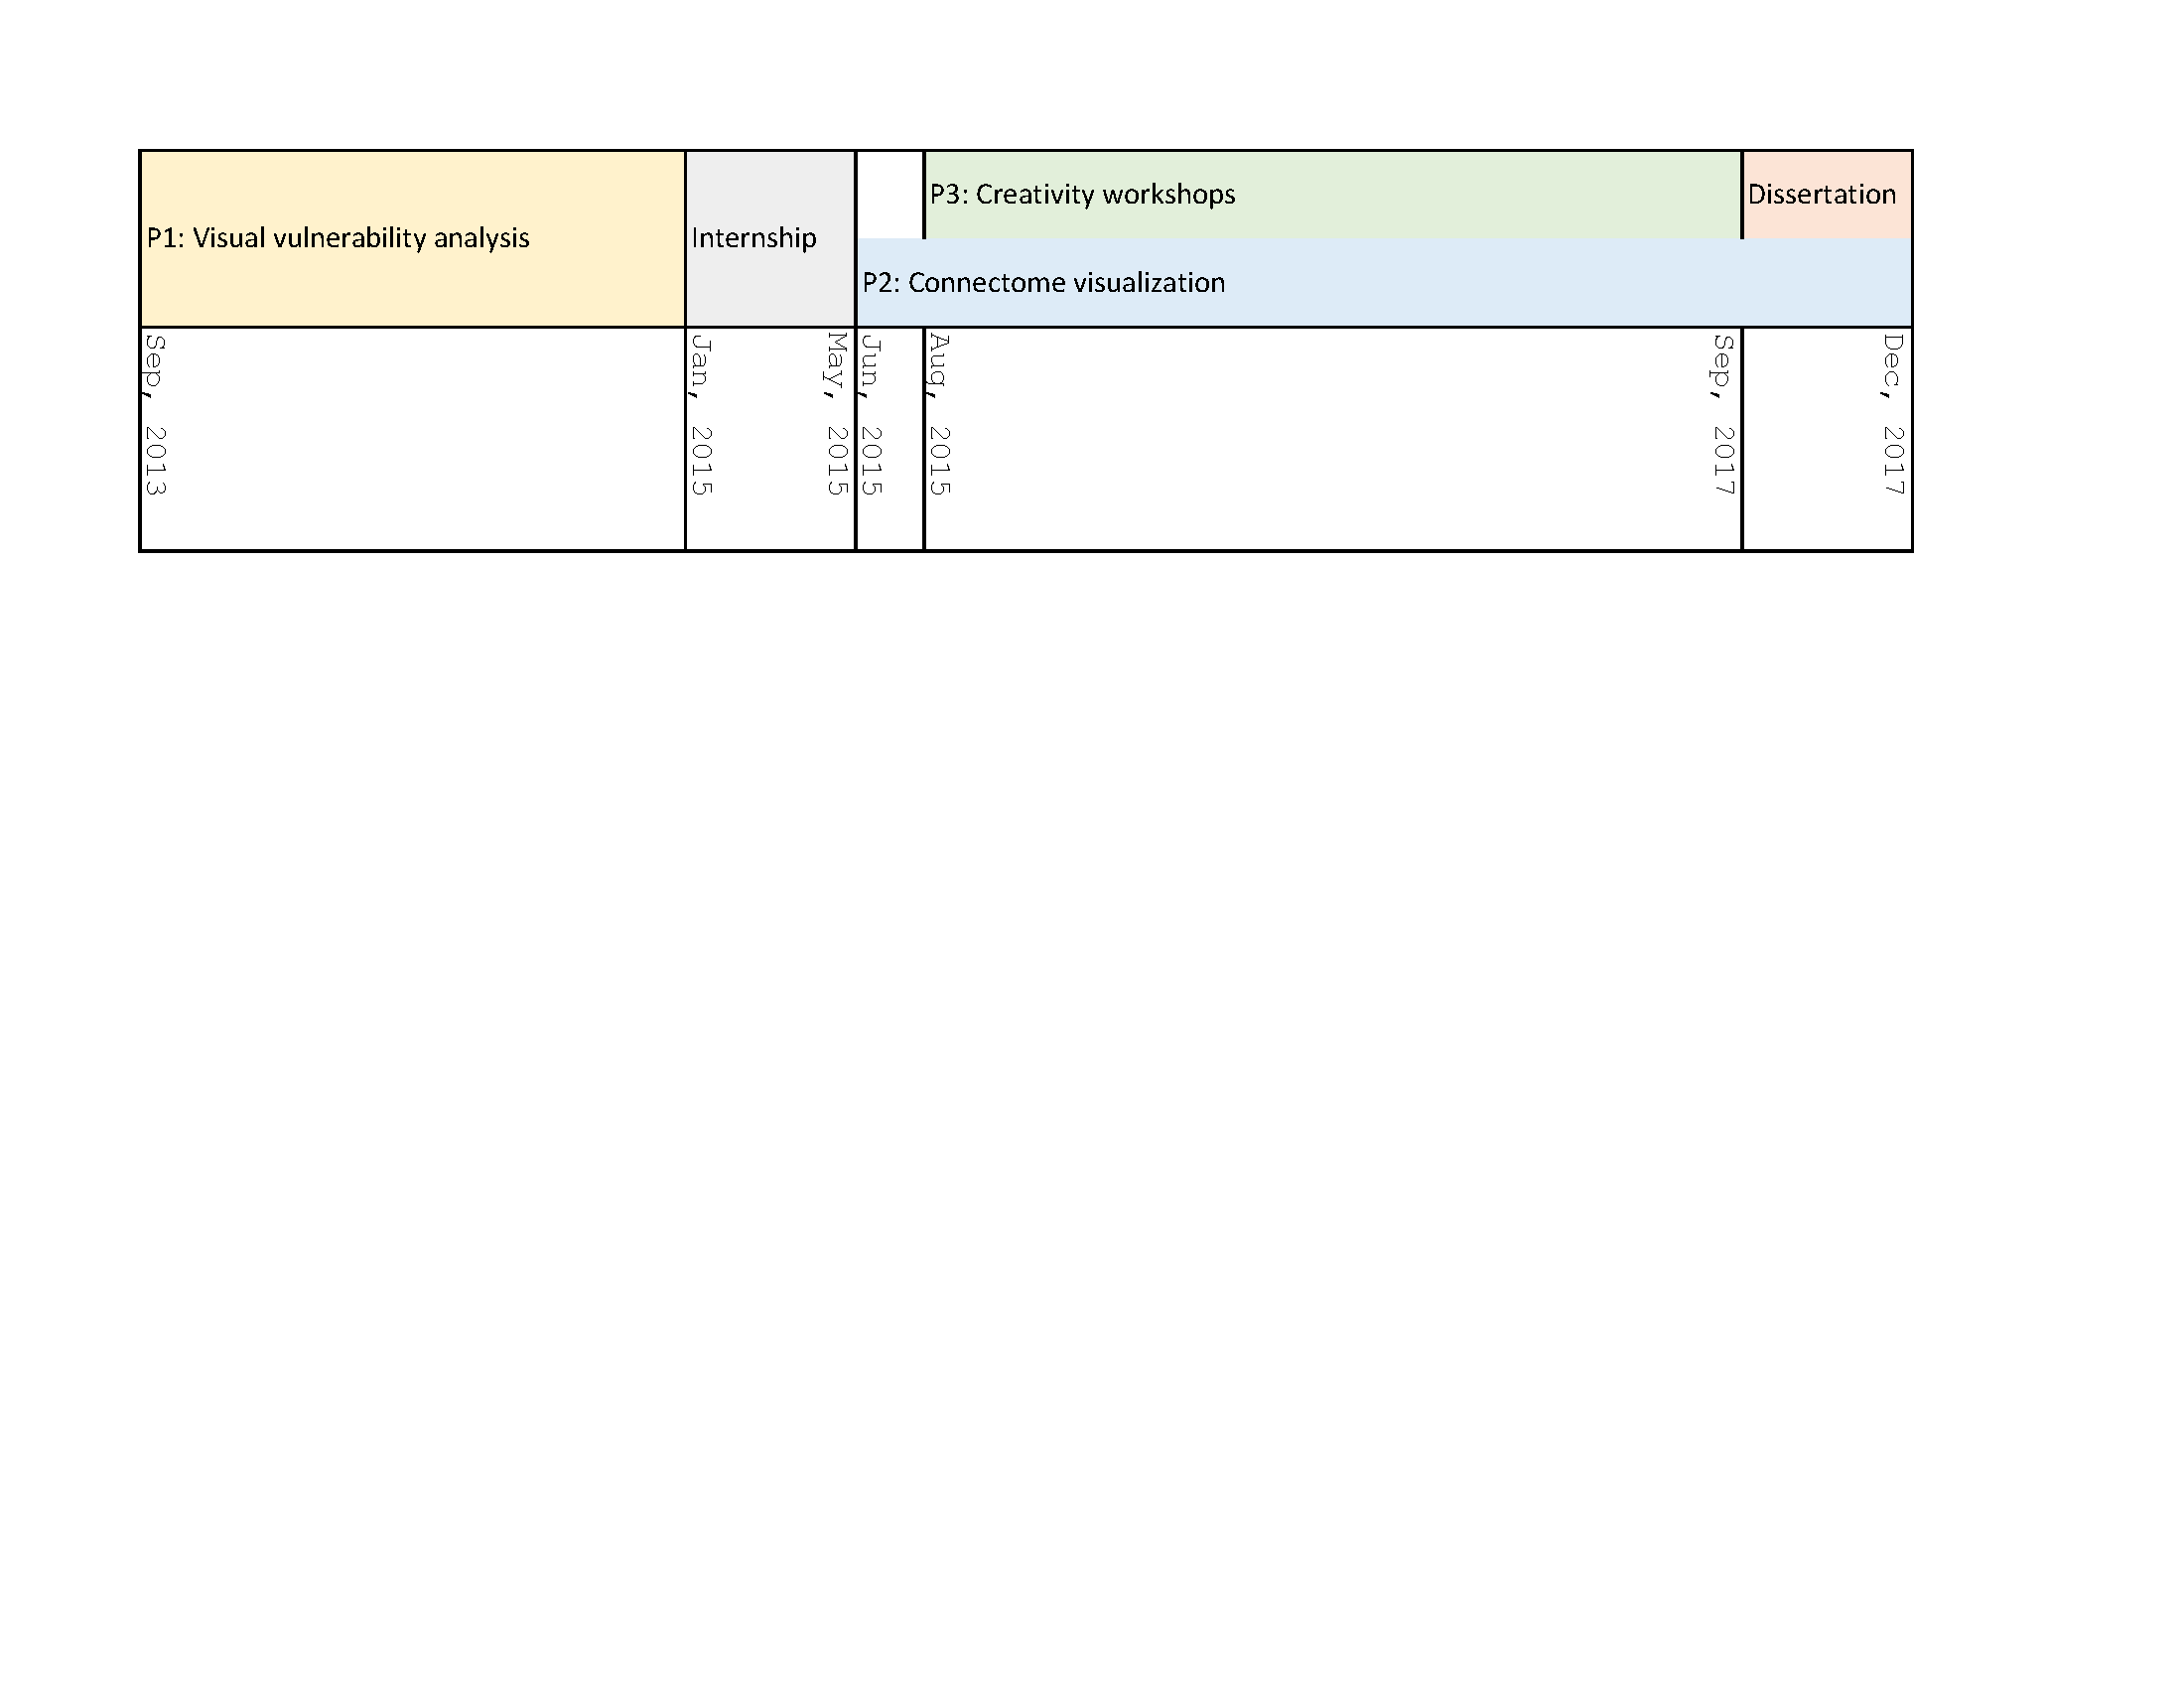
\includegraphics[width=\linewidth,trim={1cm 15cm 2cm 0}]{sources/figures/06_timeline}
  %\caption{Timeline our completed and proposed work spanning the last four years. We propose completing the visualization creativity workshop framework by September, 2017.}
%\label{fig:06_timeline}
%\end{figure}

% \numberofappendices = 1   % Set 0 for none, else number of appendices.
\numberofappendices = 3
\appendix       % Chapters, sections are now appendix style A, A.1, A.2, B, C, D, ...

%\include {sources/appa}
%\include {sources/appb}
%\include {sources/appc}

%%% The choice of bibliography style is a major decision, jointly made
%%% by you, your thesis advisor and the thesis editor. Common choices are
%%% one of the four standard BibTeX styles (abbrv, alpha, plain, and unsrt),
%%% or enhanced styles like acm, amsplain, siam, and hundreds of others
%%% available in TeX Live, and other Unix and Windows TeX distributions.
%%%
%%% Do NOT handcode your reference list, because you are unlikely to
%%% achieve consistency or conformance to the University of Utah Thesis Office
%%% requirements: let BibTeX do that tedious job for you!
%%%
%%% Remember that reference-list metadata in BibTeX files remains
%%% constant across journals and publishers, and is are often reused
%%% in other documents and shared with others, whereas formatted
%%% reference-list styles change: with BibTeX, you only need to record
%%% the metadata once.
%%%
%%% If you prefer named, rather than numeric or tagged citations, you
%%% may use styles such as authordate{1,2,3,4}, chicago, harvard, or
%%% natbib.  Be aware, however, that most of those require an
%%% additional \usepackage{} command to supply \LaTeX{} with
%%% definitions of commands that the style needs, and that there are
%%% usually several flavors of LaTeX citation commands beyond the
%%% standard \cite{} command that you need to understand before you
%%% can use them properly in your prose.

%%% This tells BibTeX to read siam.bst from the first directory where
%%% it is found in the BSTINPUTS search path:

\bibliographystyle{abbrv}

%%% This can also specify a comma-separated list (without embedded
%%% spaces) of *.bib files found by BibTeX in its BIBINPUTS search
%%% path.  The argument \jobname means the base name of the top-level
%%% LaTeX file, avoiding an unnecessary filename dependence here.
%%%
%%% BibTeX writes only one .bbl file, no matter how many *.bib files
%%% are listed here, using the name \jobname.bbl.
%%%
%%% LaTeX reads BibTeX's formatted reference list from the file
%%% \jobname.bbl.

\bibliography{mendeley}

\end {document}
